\chapter{Analisi del sistema}\label{cha:analisi}

\section{Introduzione}
In questo documento effetturemo l'analisi del sistema, ci avvarremo del linguaggio \gls{uml} per formalizzare i requisiti descritti nel documento \docref{cha:specifica_requisiti} e in parte espressi nei casi d'uso nella \docref{cha:usecase}.
Effettueremo la formalizzazione esclusivamente delle parti prinicpali del sistema, in particolare andremo a realizzare i seguenti diagrammi:
\begin{itemize}
	\item \nameref{cha:attivita}
	\item \nameref{cha:package}
	\item \nameref{cha:classi}
	\item \nameref{cha:sequenza}
\end{itemize}
Per capire come strutturare le classi, le interazioni tra di esse e le operazioni che devono svolgere, utilizzeremo le carte \gls{crc}.

\section{Diagrammi di attività} \label{cha:attivita}
I diagrammi di attività descrivono il comportamento nel tempo di un particolare elemento. Con essi si modella l’interazione e la fusione dei flussi principali con i flussi alternativi dei casi d’uso. Questo viene fatto per rendere più visibili le varie ramificazioni che i flussi possono avere all’interno di un caso d’uso. Di seguito sono elencati i diagrammi di attività, non verranno riportati tutti i diagrammi, ma solo quelli corrispondenti ai casi d'uso principali.
\begin{center}
	\begin{tabularx}{\textwidth}{ l X } 
		\toprule
		\formattaTitoloTab{ID} & \formattaTitoloTab{Caso d'uso di riferimento} \\
		\cmidrule(l{\cmidrulekern}r{\cmidrulekern}){1-2}
		\newAttivita{da:login}{\formattaAT}{Login} & \getIDTitletodesc{cu:login} \\ 
		\addlinespace[1em] 
		\newAttivita{da:logout}{\formattaAT}{Logout} & \getIDTitletodesc{cu:logout} \\ 
		\addlinespace[1em] 
		\newAttivita{da:iscrizione}{\formattaAT}{Iscrizione} & \getIDTitletodesc{cu:iscrizionePortale} \\
		 													 & \getIDTitletodesc{cu:iscrizioneSocial} \\
															 & \getIDTitletodesc{cu:iscrizioneApprovazione} \\ 
		\addlinespace[1em] 
		\newAttivita{da:approvazione}{\formattaAT}{Approvazione iscrizione} & \getIDTitletodesc{cu:approvazioneIscrizione} \\ 
		\addlinespace[1em]
		\newAttivita{da:schedaprodotto}{\formattaAT}{Inserimento scheda prodotto} & \getIDTitletodesc{cu:personalizzaVetrinaInsProd} \\
		\addlinespace[1em]
		\newAttivita{da:ricerche}{\formattaAT}{Ricerche} & \getIDTitletodesc{cu:ricercaProdotto} \\
														 & \getIDTitletodesc{cu:ricercaNotizia} \\
														 & \getIDTitletodesc{cu:ricercaProfilo} \\
		\addlinespace[1em]
		\newAttivita{da:valrec}{\formattaAT}{Inserimento valutazione e recensione} & \getIDTitletodesc{cu:inserisciValutazioneProdotto} \\
																				   & \getIDTitletodesc{cu:inserisciRecensioneProdotto}\\
		\addlinespace[1em]
		\newAttivita{da:oprec}{\formattaAT}{Operazioni recensione} & \getIDTitletodesc{cu:modificaRecensioneProdotto}\\
																   & \getIDTitletodesc{cu:eliminaRecensioneProdotto}\\
																   & \getIDTitletodesc{cu:commentoRecensione}\\
																   & \getIDTitletodesc{cu:giudizioRecensione}\\ 
																   & \getIDTitletodesc{cu:modificaGiudizioRecensione}\\ 
		\bottomrule
	\end{tabularx}
\end{center}

\linkedSubsection{da:login}
\begin{center}
			\includegraphics[width=\textwidth]{assets/visualParadigm/attivita/login}
\end{center}

\linkedSubsection{da:logout}
\begin{center}
	\includegraphics[width=\textwidth]{assets/visualParadigm/attivita/logout}
\end{center}

\linkedSubsection{da:iscrizione}
\begin{center}
	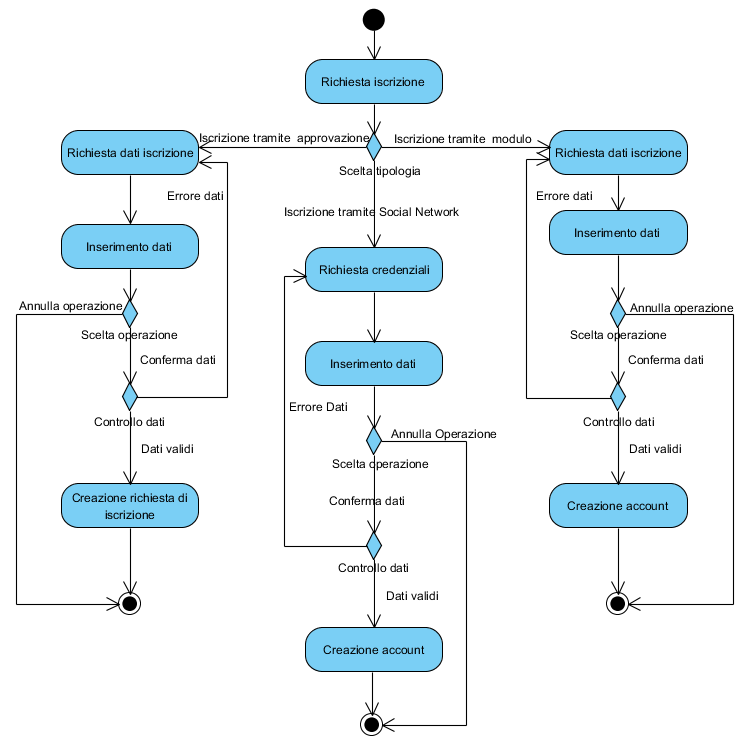
\includegraphics[width=\textwidth]{assets/visualParadigm/attivita/iscrizioni}
\end{center}

\linkedSubsection{da:approvazione}
\begin{center}
	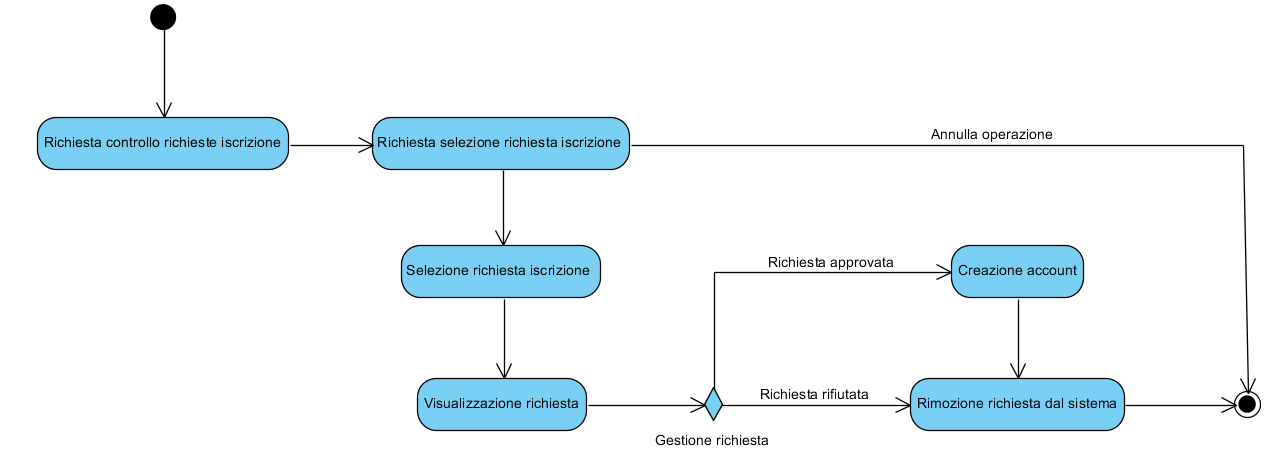
\includegraphics[width=\textwidth]{assets/visualParadigm/attivita/approvazioneIscrizione}
\end{center}

\linkedSubsection{da:schedaprodotto}
\begin{center}
	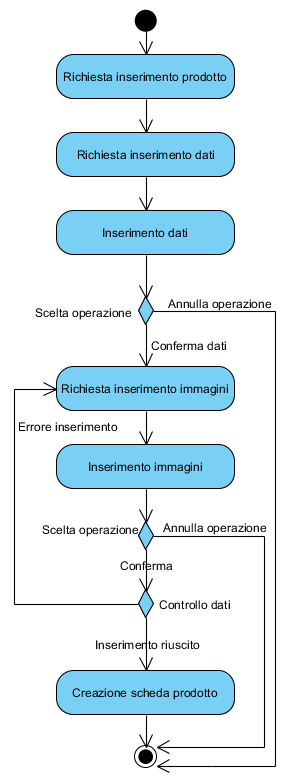
\includegraphics[width=0.5\textwidth]{assets/visualParadigm/attivita/schedaprodotto}
\end{center}

\linkedSubsection{da:ricerche}
\begin{center}
	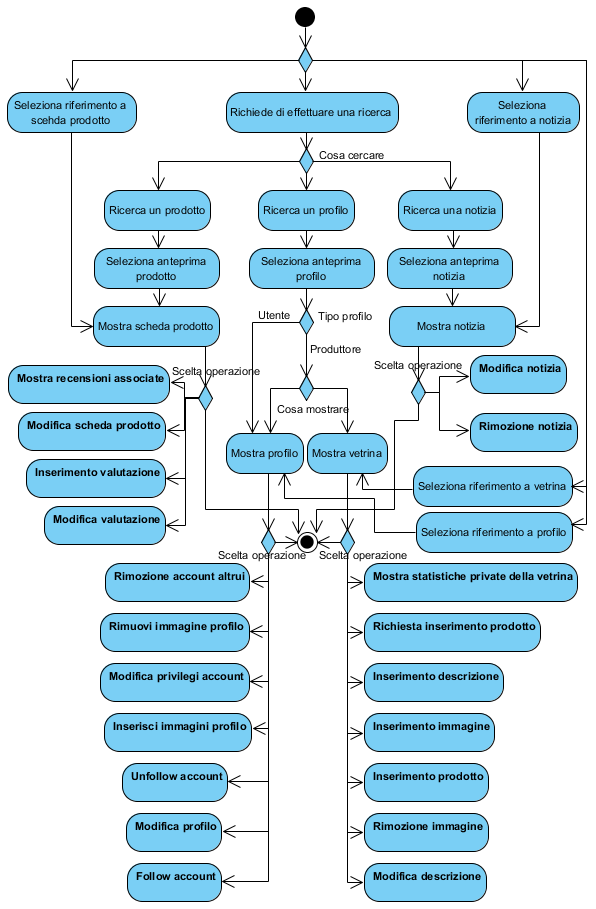
\includegraphics[width=0.94\textwidth]{assets/visualParadigm/attivita/ricerche}
\end{center}

\linkedSubsection{da:valrec}
\begin{center}
	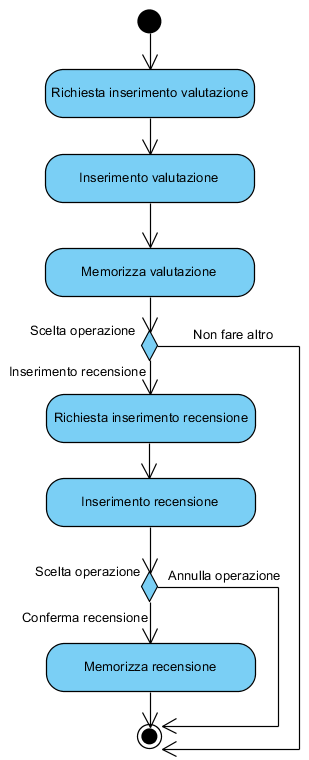
\includegraphics[width=0.5\textwidth]{assets/visualParadigm/attivita/valutazioneRecensione}
\end{center}

\linkedSubsection{da:oprec}
\begin{center}
	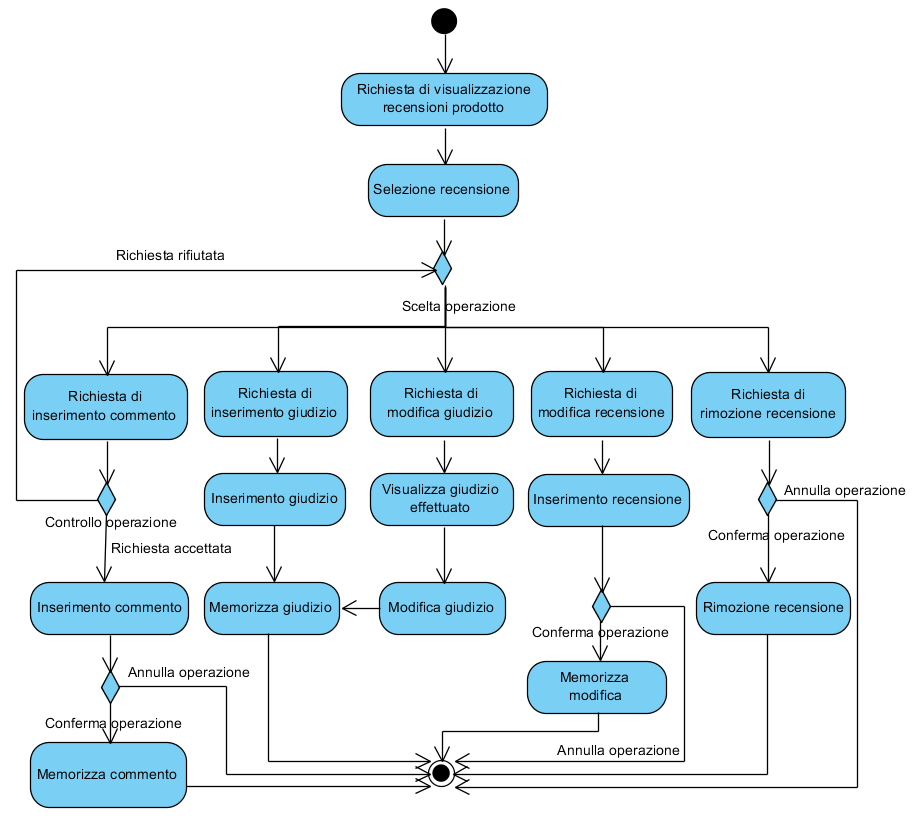
\includegraphics[width=\textwidth]{assets/visualParadigm/attivita/mostraRecensioni}
\end{center}

% \ul{testoSottolineato}
% \setulcolor{orange}
% \setul{depth}{thickness} 
%
%es.\setul{1ex}{0.8ex}
%\definecolor{orange}{rgb}{1,0.5,0}
%\setulcolor{orange}}


\section{Analisi nomi verbi} 
In questa sezione verrà effettuala l'analisi nomi/verbi della \docref{cha:specifica_sistema}.
Si utilizzeranno le seguenti convenzioni:
\begin{itemize}
	\item Una \ulR{sottolineatura rossa} indica una canditata classe
	\item Una \ulG{sottolineatura verde} indica un canditato attributo
	\item Una \ulB{sottolineatura blu} indica una canditata operazione
\end{itemize}

\subsection{Analisi della specifica del sistema} 
Il portale che si vuole realizzare interagirà con diverse \grupporuolo{figure pubbliche}, che si distinguono tra autenticate e non autenticate. Fra le \grupporuolo{figure pubbliche autenticate} troviamo gli \ruolo{utenti} e i \ruolo{produttori}, mentre i \ruolo{visitatori} sono l'unica \grupporuolo{figura pubblica non autenticata}.
Sono presenti inoltre diverse \grupporuolo{figure amministrative}, quali i \ruolo{redattori}, gli \ruolo{assistenti}, i \ruolo{moderatori} e gli \ruolo{amministratori}.
Le diverse figure presenti si distinguono a seconda di quali funzionalità possono utilizzare. 

\bigskip
\noindent

Nel sistema sono presente diversi \ulR{tipi di account}.
Ogni \ulR{account} presente nel sistema possiede almeno un \ulG{tipo} e, a seconda dei tipi che possiede, gli vengono associati determinati \ulR{privilegi}, che gli permettono l'accesso alle funzionalità che ogni privilegio fornisce. In questo modo un singolo account può ricoprire più ruoli, è ad esempio possibile che un utente sia anche un redattore anche se quest'ultimo di base non è un utente.

I \ruolo{visitatori} possono \ulB{effettuare l'iscrizione}, diversa a seconda della tipologia di account che si vuole \ulB{creare}, e \ulB{l'autenticazione}. La creazione di un \ulR{account} \ruolo{utente} può essere effettuata tramite l'integrazione con Facebook.

Gli \ruolo{utenti} possono \ulB{valutare oppure effettuare una recensione} di un \ulR{prodotto}, la quale aggiunge una \ulG{descrizione} con eventuali \ulG{immagini} alla \ulR{valutazione}. Una volta \ulB{inserita} una \ulR{recensione} o una \ulR{valutazione} è possibile \ulB{modificarla}, oppure è possibile \ulB{eliminare} la propria \ulR{recensione}. 
Per permettere di \ulB{visualizzare} velocemente le \ulR{recensioni} più utili, gli \ruolo{utenti} possono \ulB{dare} un \ulR{giudizio} \ulG{positivo} oppure \ulG{negativo} alle \ulR{recensioni} presenti. Hanno inoltre la possibilità di \ulB{commentare} le \ulR{recensioni}, per permettere una maggiore interazione fra gli \ruolo{utenti}.
Per facilitare l'inserimento di informazioni nel portale sono state inoltre pensate due particolari funzionalità: l'\ruolo{utente} può \ulB{suggerire un prodotto mancante ad un produttore iscritto}, e tale \ruolo{produttore} potrà scegliere se \ulB{accettare o rifiutare} la \ulR{richiesta di inserimento}, eventualmente modificando le \ulG{informazioni} inserite dall'\ruolo{utente}; inoltre l'\ruolo{utente} potrà \ulB{suggerire al sistema un prodotto mancante di un produttore esterno non ancora iscritto} al portale.

I \ruolo{produttori} hanno a disposizione uno spazio per pubblicizzare i loro prodotti, che da questo momento in avanti chiameremo \ulR{vetrina}. Essi potranno \ulB{personalizzare} la loro \ulR{vetrina}, \ulB{inserendo} una \ulG{descrizione} e un \ulG{immagine}. Potranno \ulB{inserire prodotti o modificare quelli già inseriti}. L'inserimento di prodotti seguirà una rigida procedura per garantire la consistenza dei dati e facilitare la \ulB{ricerca dei prodotti}. Potranno inoltre \ulB{commentare le recensioni} dei prodotti.

\bigskip
Le \grupporuolo{figure pubbliche autenticate} possono usufruire del sistema di \ulG{follower/followed}, possono quindi \ulB{seguire altri account} per \ulB{ricevere aggiornamenti} da essi, \ulB{rimuovere account} che si stanno seguendo oppure \ulB{visualizzare gli aggiornamenti dagli account seguiti}. Possono inoltre \ulB{segnalare recensioni/commenti con contenuti non appropriati} e \ulB{aprire} \ulR{ticket} per richiedere assistenza.

I \ruolo{visitatori} e gli \ruolo{utenti} possono \ulB{ricevere consigli} sui prodotti o sulle notizie simili a quelli che stanno visualizzando. 

Tutte le \grupporuolo{figure pubbliche} possono \ulB{effettuare ricerche} nel portale, in base a diversi criteri, di \ulR{prodotti}, di \ulR{notizie} e di \ulR{profili pubblici}.
Esse possono inoltre \ulB{gestire il proprio account}, con la possibilità di \ulB{visualizzare il profilo} (pubblico), \ulB{accedere alle impostazioni} (private), effettuare il \ulB{logout} oppure \ulB{rimuovere l'account}. Da notare che l'eventuale \ulB{rimozione dell'account} non comporterà la rimozione dei contenuti inseriti nel portale, ma solo la rimozione dello stesso. Possono inoltre \ulB{visualizzare} i \ulR{contenuti} pubblici del portale, quali le \ulR{vetrine} dei produttori, i singoli \ulR{prodotti} con le \ulR{recensioni} associate, i \ulR{profili pubblici} e le \ulR{notizie} presenti nel portale.

\bigskip
\noindent
Segue una descrizione delle funzionalità specifiche delle \grupporuolo{figure amministrative}.

I \ruolo{redattori} possono \ulB{aggiungere}, \ulB{modificare} o \ulB{rimuovere} \ulR{notizie} provenienti dal mondo dolciario.

Gli \ruolo{assistenti} possono \ulB{rispondere} ai \ulR{ticket} per risolvere i problemi degli \ruolo{utenti}. Hanno inoltre il compito di \ulB{gestire le iscrizioni} dei produttori effettuate direttamente nel portale, controllando la veridicità delle informazioni inserite, ed in caso \ulB{creare l'account} richiesto.

I \ruolo{moderatori} possono \ulB{eliminare contenuti non appropriati} presenti nel sistema, che possono essere \ulB{segnalati} dalle \grupporuolo{figure pubbliche autenticate}.

Gli \ruolo{amministratori} possono accedere al pannello di controllo del \gls{cms}, attraverso il quale possono configurare il portale in ogni suo aspetto. Può inoltre gestire gli account, \ulB{creandone di nuovi, modificando i privilegi o rimuovendo} quelli già presenti. 

\bigskip
\noindent
Nel portale che si vuole realizzare le informazioni sui \ulR{prodotti} sono di fondamentale importanza, perciò elenchiamo di seguito quelle contenute nel sistema:
\begin{itemize}
	\item \infoProdotto{\ulG{Nome prodotto.}}
	\item \infoProdotto{\ulG{Descrizione di presentazione.}}
	\item \infoProdotto{\ulG{Almeno un'immagine del prodotto.}}
	\item \infoProdotto{\ulG{Marca.}}
	\item \infoProdotto{\ulG{Categoria.}}
	\item \infoProdotto{\ulG{Consistenza.}}
	\item \infoProdotto{\ulG{Particolarità.}}
	\item \infoProdotto{\ulG{Ingredienti.}}
\end{itemize}
L'inserimento di queste informazioni è compito del \ruolo{produttore}, il quale seguirà una rigida procedura che sarà descritta nel dettaglio durante la specifica delle funzionalità.


\section{Carte CRC}
Le carte \gls{crc} sono uno strumento usato per impostare un progetto software object-oriented attraverso un processo di brainstorming.
Ciascuna carta descrive una classe in modo sommario, indicando:
\begin{itemize}
	\item Il nome della classe
 	\item Le sue superclassi
 	\item Le sue sottoclassi
 	\item Le sue responsabilità
 	\item Le sue collaborazioni
\end{itemize}
Dove le sue collaborazioni sono altre classi con cui essa collabora per svolgere i compiti di cui è responsabile
Di seguito sono elencate le carte \gls{crc}:
\begin{itemize}%{key}{nome}{superclassi}{sottoclassi}
	\item \newClassItem{class:GestioneIscritti}{Gestione iscritti}{\noClasse}{\noClasse}
	\item \newClassItem{class:RichiestaIscrizione}{Richiesta Iscrizione}{\noClasse}{\noClasse}
	\item \newClassItem{class:Account}{Account}{\noClasse}{\noClasse}
	\item \newClassItem{class:TipoAccount}{Tipo Account}{\noClasse}{\noClasse}
	\item \newClassItem{class:Privilegi}{Privilegi}{\noClasse}{\noClasse}
	\item \newClassItem{class:Contenuto}{Contenuto}{\noClasse}{\getTitletodesc{class:Commento}, \getTitletodesc{class:Recensione}, \getTitletodesc{class:Giudizio}, \getTitletodesc{class:Scheda Prodotto}, \getTitletodesc{class:Valutazione}, \getTitletodesc{class:Notizia}}
	\item \newClassItem{class:Commento}{Commento}{\getTitletodesc{class:Contenuto}}{\noClasse}
	\item \newClassItem{class:Recensione}{Recensione}{\getTitletodesc{class:Contenuto}}{\noClasse}
	\item \newClassItem{class:Giudizio}{Giudizio}{\getTitletodesc{class:Contenuto}}{\noClasse}
	\item \newClassItem{class:Scheda Prodotto}{Scheda Prodotto}{\getTitletodesc{class:Contenuto}}{\noClasse}
	\item \newClassItem{class:Valutazione}{Valutazione}{\getTitletodesc{class:Contenuto}}{\noClasse}
	\item \newClassItem{class:Notizia}{Notizia}{\getTitletodesc{class:Contenuto}}{\noClasse}
	\item \newClassItem{class:ConsistenzaProdotto}{Consistenza Prodotto}{\noClasse}{\noClasse}
	\item \newClassItem{class:CategoriaProdotto}{Categoria Prodotto}{\noClasse}{\noClasse}
	\item \newClassItem{class:Ticket}{Ticket}{\noClasse}{\getTitletodesc{class:RichiestaProduttore}}
	\item \newClassItem{class:RichiestaProduttore}{Richiesta Produttore}{\getTitletodesc{class:Ticket}}{\noClasse}
	\item \newClassItem{class:RispostaTicket}{Risposta Ticket}{\noClasse}{\noClasse}
	\item \newClassItem{class:RichiestaProdotto}{Richiesta Prodotto}{\noClasse}{\noClasse}
	\item \newClassItem{class:GestioneSegnalazioni}{Gestione Segnalazioni}{\noClasse}{\noClasse}
	\item \newClassItem{class:SegnalazioneContenuto}{Segnalazione Contenuto}{\noClasse}{\noClasse}
	\item \newClassItem{class:Profilo}{Profilo}{\noClasse}{\getTitletodesc{class:ProfiloProduttore}}
	\item \newClassItem{class:ProfiloProduttore}{Profilo Produttore}{\getTitletodesc{class:Profilo}}{\noClasse}
	\item \newClassItem{class:Vetrina}{Vetrina}{\noClasse}{\noClasse}
	\item \newClassItem{class:Gestione Accessi}{Gestione Accessi}{\noClasse}{\noClasse}
	\item \newClassItem{class:Accesso Iscritto}{Accesso Iscritto}{\noClasse}{\noClasse}
	\item \newClassItem{class:Accesso Ospite}{Accesso Ospite}{\noClasse}{\noClasse}
	\item \newClassItem{class:Utility}{Utility}{\noClasse}{\getTitletodesc{class:Ricerca}}
	\item \newClassItem{class:Ricerca}{Ricerca}{\getTitletodesc{class:Utility}}{\noClasse}
	\item \newClassItem{class:TipoRicerca}{Tipo Ricerca}{\noClasse}{\noClasse}
	\item \newClassItem{class:Anteprima}{Anteprima}{\noClasse}{\getTitletodesc{class:AnteprimaProdotto}, \getTitletodesc{class:AnteprimaProfilo}, \getTitletodesc{class:AnteprimaNotizia}}
	\item \newClassItem{class:AnteprimaProdotto}{Anteprima Prodotto}{\getTitletodesc{class:Anteprima}}{\noClasse}
	\item \newClassItem{class:AnteprimaProfilo}{Anteprima Profilo}{\getTitletodesc{class:Anteprima}}{\getTitletodesc{class:AnteprimaProfiloProduttore}}
	\item \newClassItem{class:AnteprimaProfiloProduttore}{Anteprima Profilo Produttore}{\getTitletodesc{class:AnteprimaProfilo}}{\noClasse}
	\item \newClassItem{class:AnteprimaNotizia}{Anteprima Notizia}{\getTitletodesc{class:Anteprima}}{\noClasse}
\end{itemize}

\crcTab{class:GestioneIscritti}
{\begin{itemWork}
	\item Signleton necessario per raccogliere tutte le informazioni riguardanti le iscrizioni
	\item Possibilità di effettuare l'iscrizione
\end{itemWork}}
{\begin{itemWork}
	\item Account
\end{itemWork}}

\vspaceTab

\crcTab{class:RichiestaIscrizione}
{\begin{itemWork}
	\item Memorizzazione delle informazioni necessarie per la creazione di una richiesta di iscrizione
\end{itemWork}}
{\begin{itemWork}
	\item Account
\end{itemWork}}

\vspaceTab

\crcTab{class:Account}
{\begin{itemWork}
	\item Memorizzazione delle informazioni account
\end{itemWork}}
{\begin{itemWork}
	\item Tipo account, Profilo
\end{itemWork}}

\vspaceTab

\crcTab{class:TipoAccount}
{\begin{itemWork}
	\item Enumerazione delle possibili tipologie di account presenti nel sistema
	\item Possibilità di ottenere i privilegi disponibili dati i tipi posseduti
\end{itemWork}}
{\begin{itemWork}
	\item Privilegi
\end{itemWork}}

\vspaceTab

\crcTab{class:Privilegi}
{\begin{itemWork}
	\item Enumerazione dei possibili privilegi, per avere accesso alle diverse funzionalità, che un account può avere
\end{itemWork}}
{-}

\vspaceTab

\crcTab{class:Contenuto}
{\begin{itemWork}
	\item Generalizzazione dei vari tipi di contenuti presenti nel sistema
	\item Memorizzazione dell'autore del contenuto
\end{itemWork}}
{\begin{itemWork}
	\item Account
\end{itemWork}}

\vspaceTab

\crcTab{class:Commento}
{\begin{itemWork}
	\item Memorizzazione delle informazioni necessarie per commentare una recensione
\end{itemWork}}
{\begin{itemWork}
	\item Account
\end{itemWork}}

\vspaceTab

\crcTab{class:Recensione}
{\begin{itemWork}
	\item Memorizzazione delle informazioni necessarie per recensire una scheda di un prodotto
	\item Possibilità di effettuare un commento
	\item Possibilità di effettuare un giudizio
\end{itemWork}}
{\begin{itemWork}
	\item Account, Commento, Giudizio
\end{itemWork}}

\vspaceTab

\crcTab{class:Giudizio}
{\begin{itemWork}
	\item Memorizzazione delle informazioni necessarie per giudicare una recensione
\end{itemWork}}
{\begin{itemWork}
	\item Account
\end{itemWork}}

\vspaceTab

\crcTab{class:Scheda Prodotto}
{\begin{itemWork}
	\item Memorizzazione di tutte le informazioni relative al prodotto
	\item Possibilità di effettuare una recensione
	\item Possibilità di effettuare una valutazione
\end{itemWork}}
{\begin{itemWork}
	\item Recensione, Valutazione, Consistenza prodotto, Categoria prodotto
\end{itemWork}}

\vspaceTab

\crcTab{class:Valutazione}
{\begin{itemWork}
	\item Memorizzazione delle informazioni necessarie per valutare una scheda prodotto
\end{itemWork}}
{\begin{itemWork}
	\item Account
\end{itemWork}}

\vspaceTab

\crcTab{class:Notizia}
{\begin{itemWork}
	\item Memorizzazione delle informazioni necessarie per l'inserimento di una notizia
\end{itemWork}}
{\begin{itemWork}
	\item Account
\end{itemWork}}

\vspaceTab

\crcTab{class:ConsistenzaProdotto}
{\begin{itemWork}
	\item Enumerazione delle possibili consistenze di un prodotto
\end{itemWork}}
{-}

\vspaceTab

\crcTab{class:CategoriaProdotto}
{\begin{itemWork}
	\item Enumerazione delle possibili categorie di un prodotto
\end{itemWork}}
{-}

\vspaceTab

\crcTab{class:Ticket}
{\begin{itemWork}
	\item Memorizzazione delle informazioni necessarie per la creazione di un ticket
\end{itemWork}}
{\begin{itemWork}
	\item Account
\end{itemWork}}

\vspaceTab

\crcTab{class:RichiestaProduttore}
{\begin{itemWork}
	\item Memorizzazione delle informazioni necessarie per la creazione di una richiesta di inserimento di un produttore mancante
\end{itemWork}}
{\begin{itemWork}
	\item Account, Scheda Prodotto
\end{itemWork}}

\vspaceTab


\crcTab{class:RispostaTicket}
{\begin{itemWork}
	\item Memorizzazione delle informazioni necessarie per rispondere ad un ticket aperto
\end{itemWork}}
{\begin{itemWork}
	\item Ticket, Account
\end{itemWork}}

\vspaceTab

\crcTab{class:RichiestaProdotto}
{\begin{itemWork}
	\item Memorizzazione delle informazioni necessarie per la creazione di una richiesta di inserimento di un prodotto mancante
\end{itemWork}}
{\begin{itemWork}
	\item Account, Scheda Prodotto, Profilo Produttore
\end{itemWork}}

\vspaceTab

\crcTab{class:GestioneSegnalazioni}
{\begin{itemWork}
	\item Singleton necessario per raccogliere tutte le segnalazioni di contenuti presenti nel sistema
\end{itemWork}}
{\begin{itemWork}
	\item Segnalazione contenuto
\end{itemWork}}

\vspaceTab

\crcTab{class:SegnalazioneContenuto}
{\begin{itemWork}
	\item Memorizzazione delle informazioni necessarie per la creazione di una segnalazione di un contenuto
\end{itemWork}}
{\begin{itemWork}
	\item Account, Contenuto
\end{itemWork}}

\vspaceTab

\crcTab{class:Profilo}
{\begin{itemWork}
	\item Memorizzazione di tutte le informazioni del profilo
	\item Memorizzazione della lista dei follower/followed del profilo
\end{itemWork}}
{\begin{itemWork}
	\item Account
\end{itemWork}}

\vspaceTab

\crcTab{class:ProfiloProduttore}
{\begin{itemWork}
	\item Memorizzazione delle informazioni relative ad un profilo produttore
	\item Possibilità di visualizzare la vetrina associata
	\item Possibilità di visualizzare le richieste prodotto a lui indirizzate
\end{itemWork}}
{\begin{itemWork}
	\item Richiesta Prodotto, Vetrina
\end{itemWork}}

\vspaceTab

\crcTab{class:Vetrina}
{\begin{itemWork}
    \item Memorizzazione delle informazioni e dei prodotti presenti nella vetrina di un dato produttore
	\item Possibilità di gestire prodotti
\end{itemWork}}
{\begin{itemWork}
	\item Profilo Produttore, Scheda Prodotto
\end{itemWork}}

\vspaceTab

\crcTab{class:Gestione Accessi}
{\begin{itemWork}
	\item Singleton necessario per raccogliere le informazioni relative agli accessi degli iscritti e dei visitatori
\end{itemWork}}
{\begin{itemWork}
	\item Accesso Iscritto, Accesso Ospite
\end{itemWork}}

\vspaceTab


\crcTab{class:Accesso Iscritto}
{\begin{itemWork}
	\item Memorizzazione delle informazioni relative ad un accesso di un iscritto
\end{itemWork}}
{\begin{itemWork}
	\item Account
\end{itemWork}}


\vspaceTab

\crcTab{class:Accesso Ospite}
{\begin{itemWork}
	\item Memorizzazione delle informazioni relative ad un accesso di un ospite
\end{itemWork}}
{-}

\vspaceTab

\crcTab{class:Utility}
{\begin{itemWork}
	\item Classe necessaria per raccogliere metodi statici utili al sistema
\end{itemWork}}
{-}

\vspaceTab

\crcTab{class:Ricerca}
{\begin{itemWork}
	\item Gestione ricerca
\end{itemWork}}
{TipoRicerca}

\vspaceTab

\crcTab{class:TipoRicerca}
{\begin{itemWork}
	\item Enumerazione delle tipologie di ricerca presenti nel sistema
\end{itemWork}}
{-}

\vspaceTab

\crcTab{class:Anteprima}
{\begin{itemWork}
	\item Generalizzazione delle possibili anteprime dei contenuti presenti nel sistema
\end{itemWork}}
{-}

\vspaceTab

\crcTab{class:AnteprimaProdotto}
{\begin{itemWork}
	\item Memorizzazione delle informazioni necessarie per mostrare l'anteprima di un dato prodotto
	\item Possibilità di mostrare l'anteprima del prodotto associato
\end{itemWork}}
{\begin{itemWork}
	\item Prodotto
\end{itemWork}}

\vspaceTab

\crcTab{class:AnteprimaProfilo}
{\begin{itemWork}
	\item Memorizzazione delle informazioni necessarie per mostrare l'anteprima di un dato profilo
	\item Possibilità di mostrare l'anteprima del profilo associato
\end{itemWork}}
{\begin{itemWork}
	\item Profilo
\end{itemWork}}

\vspaceTab

\crcTab{class:AnteprimaProfiloProduttore}
{\begin{itemWork}
	\item Memorizzazione delle informazioni necessarie per mostrare l'anteprima di un dato profilo produttore
	\item Possibilità di mostrare l'anteprima del profilo associato, che comprenderà la possibilità di andare sia al profilo del produtture che alla vetrina dello stesso
\end{itemWork}}
{\begin{itemWork}
	\item Vetrina
\end{itemWork}}

\vspaceTab

\crcTab{class:AnteprimaNotizia}
{\begin{itemWork}
	\item Memorizzazione delle informazioni necessarie per mostrare l'anteprima di una data notizia
	\item Possibilità di mostrare l'anteprima della notizia associata
\end{itemWork}}
{\begin{itemWork}
	\item Notizia
\end{itemWork}}


%\begin{landscape}
\section{Diagramma dei package}  \label{cha:package}
Il diagramma dei package sono diagrammi di struttura che descrive i package del sistema e le relazioni tra essi.
Un Package è uno spazio dei nomi utilizzato per raggruppare elementi che sono in relazione semantica tra loro.
\begin{center}
			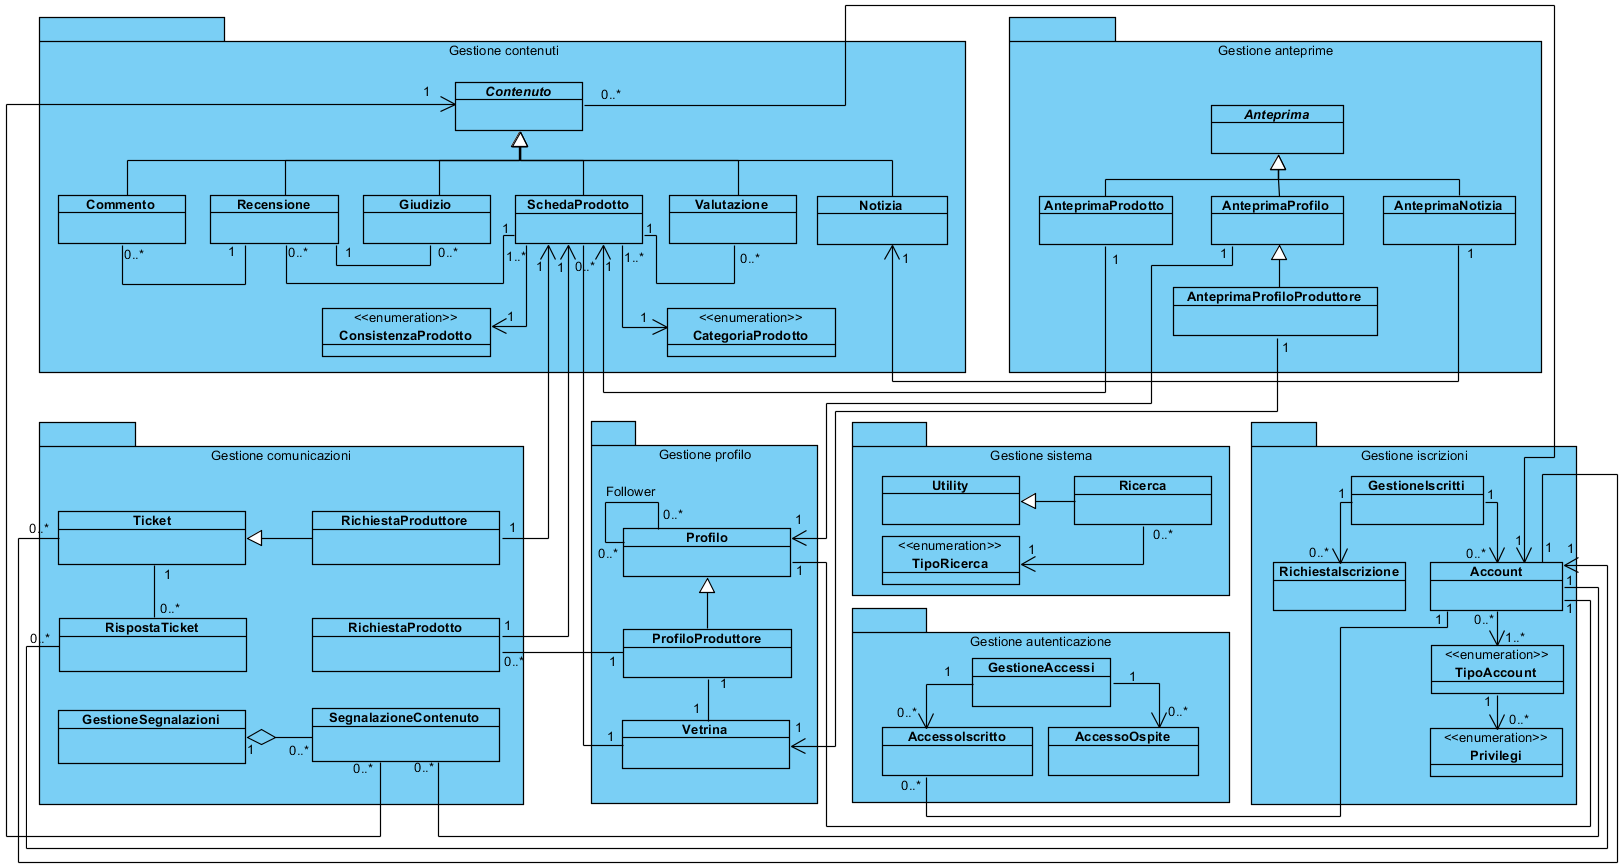
\includegraphics[width=\linewidth]{assets/visualParadigm/package/DiagrammaPacakage}
\end{center}
%\end{landscape}

\section{Diagrammi delle classi}  \label{cha:classi}
I diagrammi delle classi servono a modellare la relazione tra le entità del sistema, rappresentate come classi.
Una classe è composta da delle caratteristiche che la descrivono (attributi) e delle elaborazioni che vengono eseguite (metodi). 
Le classi servono ad identificare chi fa che cosa e come all’interno del sistema. Queste possono avere relazioni tra loro, le quali sono rappresentate con le associazioni. La cardinalità di un’associazione esprime il numero di oggetti di una certa classe che prendono parte all’associazione. Di seguito sono elencati i diagrammi delle classi:
\begin{itemize}
	\item \newPKG{pkg:GestioneAnteprime}{\formattaPKG}{Gestione anteprima}
	\item \newPKG{pkg:GestioneAutenticazione}{\formattaPKG}{Gestione autenticazione}
	\item \newPKG{pkg:GestioneIscritti}{\formattaPKG}{Gestione iscritti}
	\item \newPKG{pkg:GestioneTicket}{\formattaPKG}{Gestione ticket}
	\item \newPKG{pkg:GestioneProfilo}{\formattaPKG}{Gestione profilo}
	\item \newPKG{pkg:GestioneContenuti}{\formattaPKG}{Gestione contenuti}
	\item \newPKG{pkg:GestioneSistema}{\formattaPKG}{Gestione sistema}
\end{itemize}

\linkedSubsection{pkg:GestioneAnteprime}
\begin{center}
			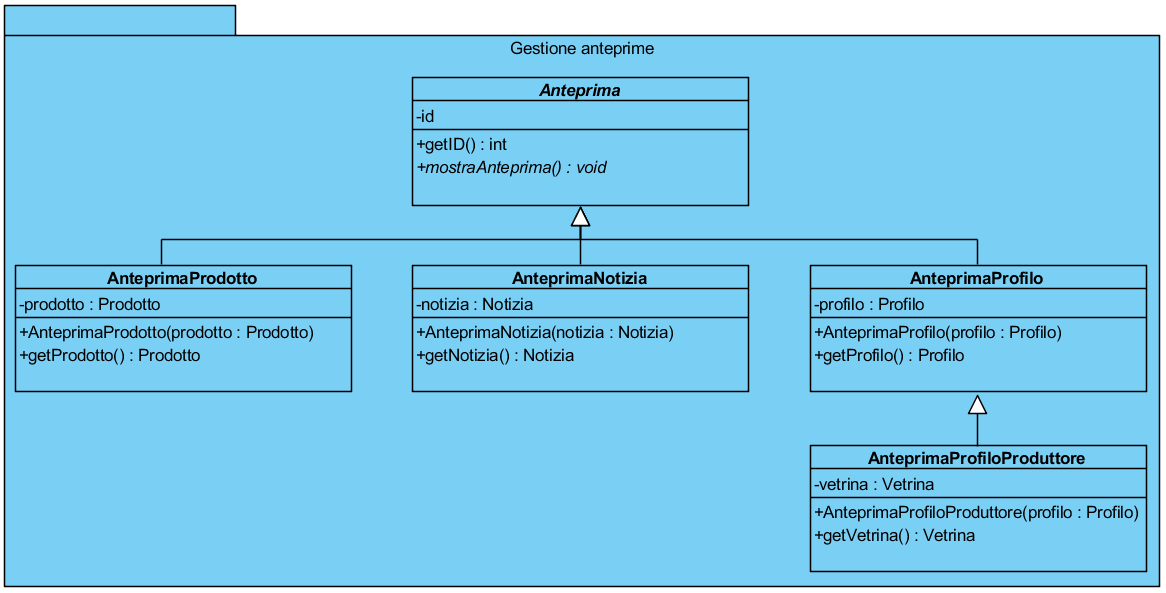
\includegraphics[width=\textwidth]{assets/visualParadigm/classi/GestioneAnteprime}
\end{center}

\linkedSubsection{pkg:GestioneAutenticazione}
\begin{center}
			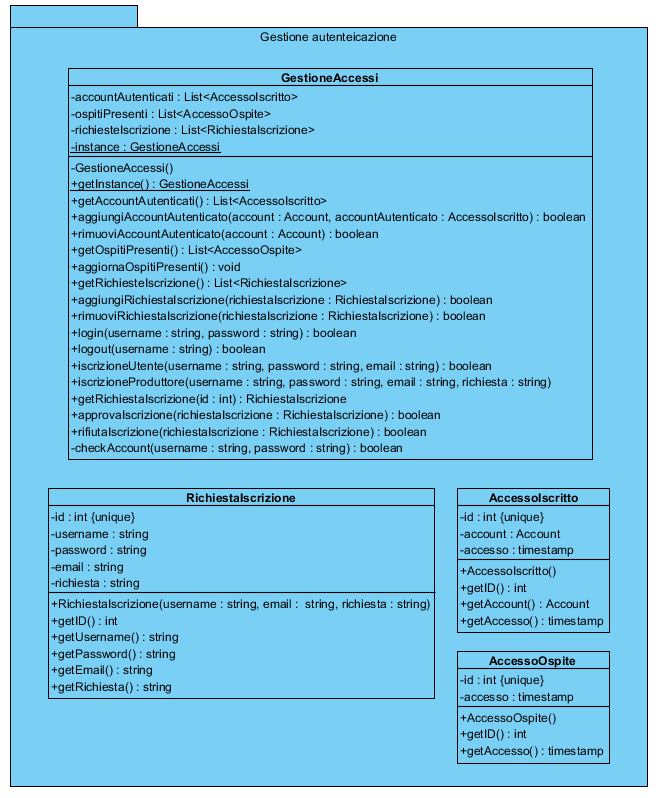
\includegraphics[width=\textwidth]{assets/visualParadigm/classi/GestioneAutenticazione}
\end{center}

\linkedSubsection{pkg:GestioneIscritti}
\begin{center}
			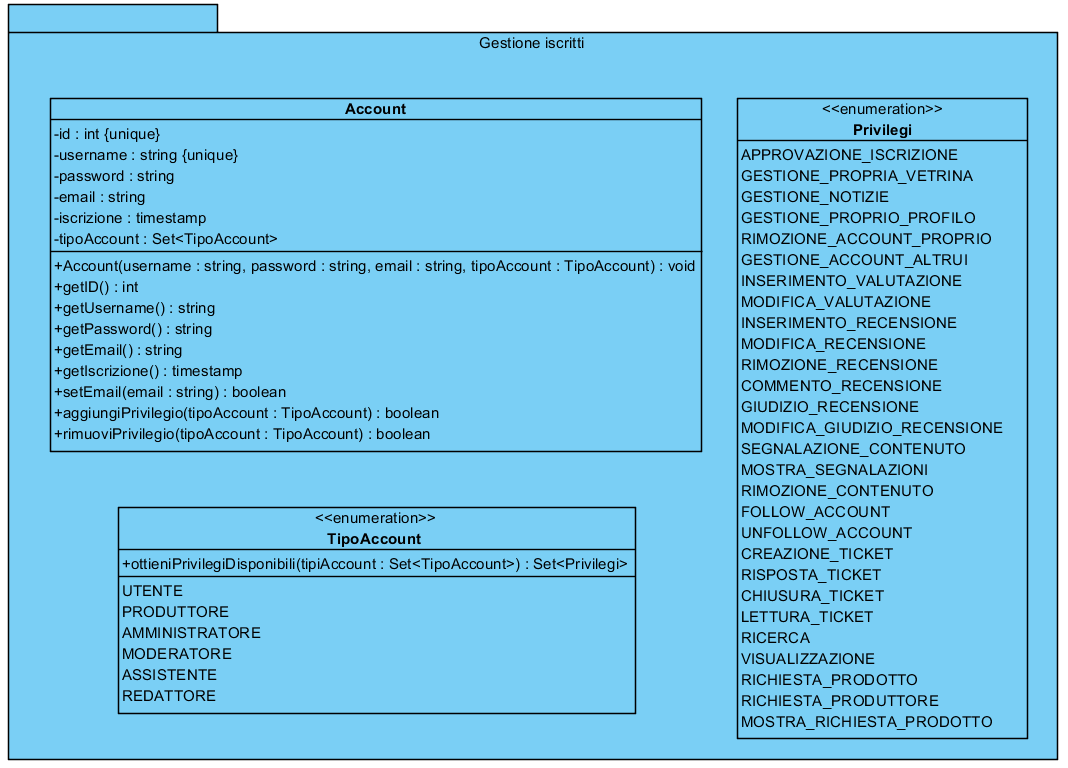
\includegraphics[width=\textwidth]{assets/visualParadigm/classi/GestioneIscritti}
\end{center}

\linkedSubsection{pkg:GestioneTicket}
\begin{center}
			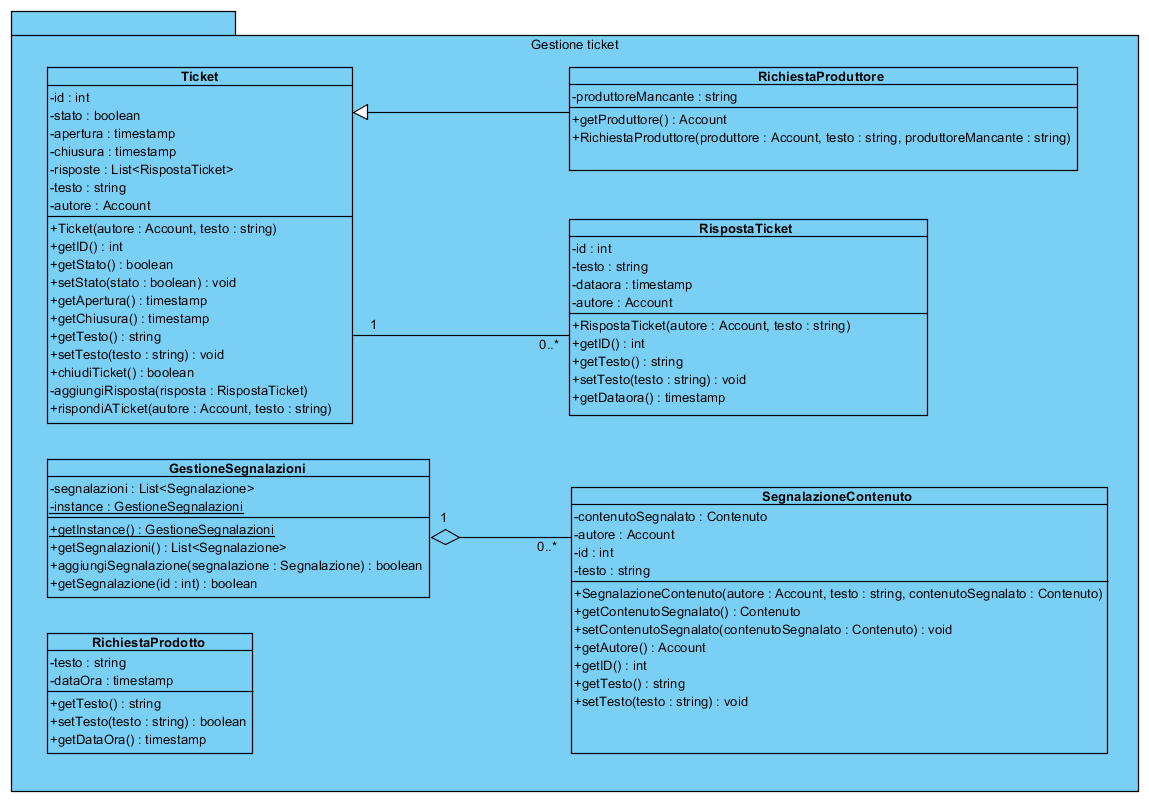
\includegraphics[width=\textwidth]{assets/visualParadigm/classi/GestioneTicket}
\end{center}

\begin{landscape}
\linkedSubsection{pkg:GestioneProfilo}
\begin{center}
			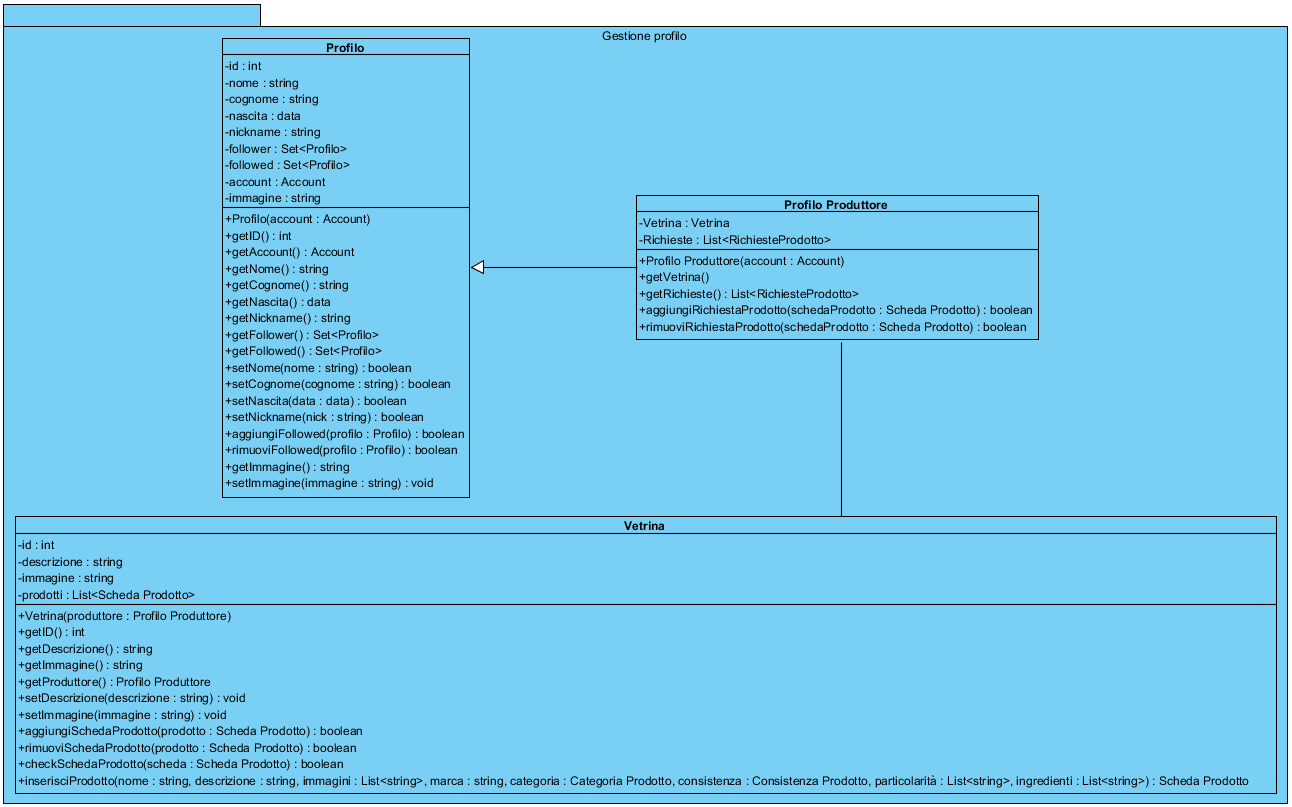
\includegraphics[width=\linewidth]{assets/visualParadigm/classi/GestioneProfilo}
\end{center}
\end{landscape}

\begin{landscape}
\linkedSubsection{pkg:GestioneContenuti}
\begin{center}
			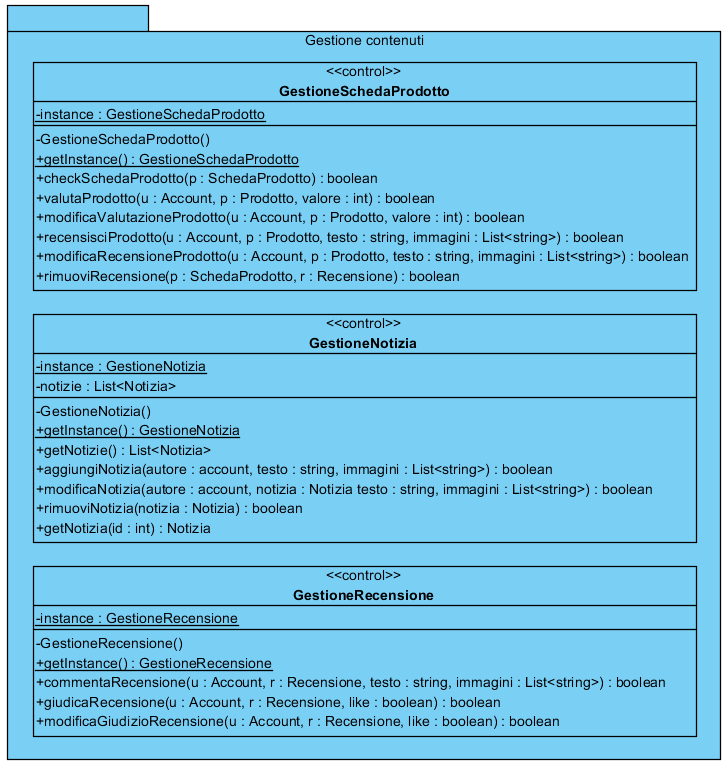
\includegraphics[width=1.1\linewidth]{assets/visualParadigm/classi/GestioneContenuti}
\end{center}
\end{landscape}

\linkedSubsection{pkg:GestioneSistema}
\begin{center}
			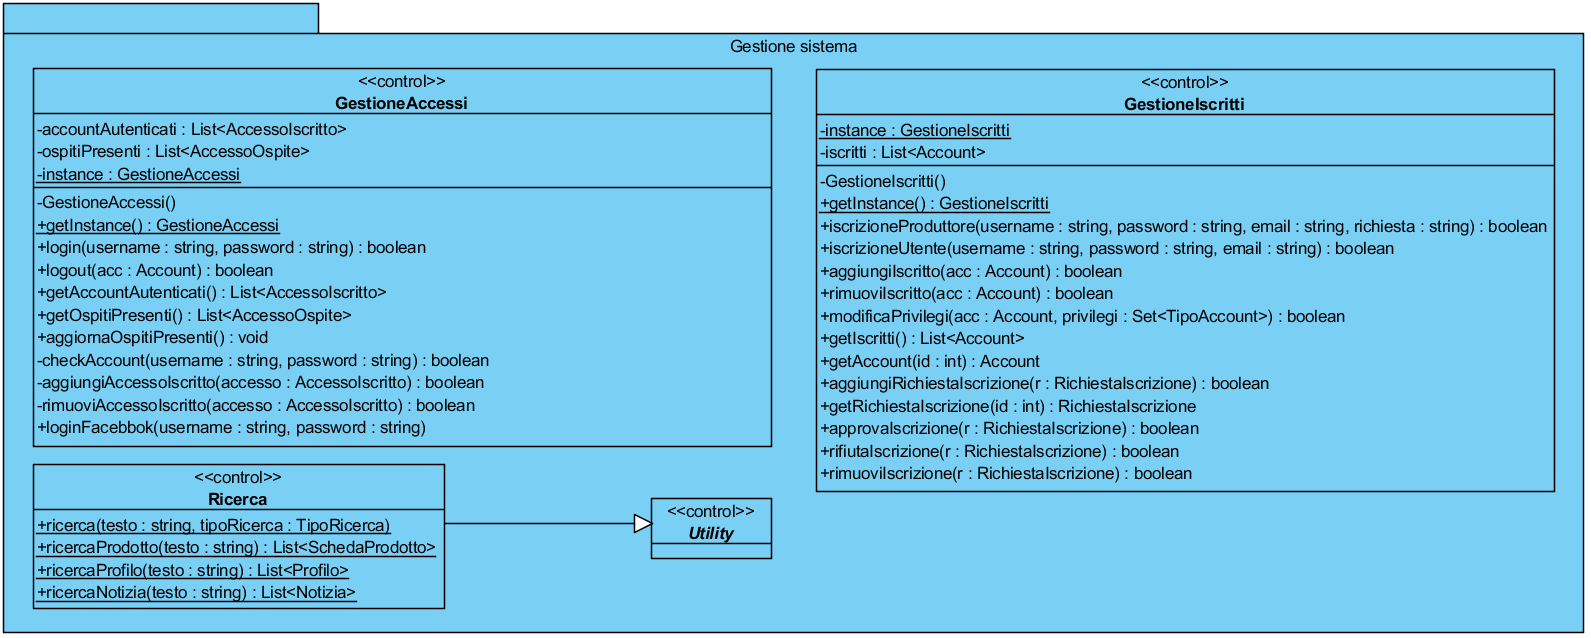
\includegraphics[width=\textwidth]{assets/visualParadigm/classi/GestioneSistema}
\end{center}


\section{Diagrammi di sequenza}  \label{cha:sequenza}
I diagrammi di sequenza descrivono le interazioni tra gli oggetti organizzate in sequenza temporale. Ogni caso d’uso contiene al suo interno diversi diagrammi di sequenza. Rappresenteremo solo le sequenze principali.
Un diagramma di sequenza è costituito da:
\begin{itemize}
	\item Gli oggetti
	\item I messaggi attraverso cui essi interagiscono
\end{itemize}
Di seguito sono elencati i diagrammi di sequenza, non verranno riportati tutti i diagrammi di sequenza, ma solo quelli corrispondenti ai casi d'uso principali.
\begin{itemize}
	\item \newSequenza{seq:login}{\formattaSEQ}{Login}
	\item \newSequenza{seq:logout}{\formattaSEQ}{Logout}
	\item \newSequenza{seq:iscrizioneProduttore}{\formattaSEQ}{Iscrizione Produttore}
	\item \newSequenza{seq:iscrizioneUtente}{\formattaSEQ}{Iscrizione Utente}
	\item \newSequenza{seq:approvazioneIscrizione}{\formattaSEQ}{Approvazione iscrizione}
	\item \newSequenza{seq:inserimentoSchedaProdotto}{\formattaSEQ}{Inserimento scheda prodotto}
	\item \newSequenza{seq:inserimentoValutazione}{\formattaSEQ}{Inserimento valutazione}
	\item \newSequenza{seq:inserimentoRecensione}{\formattaSEQ}{Inserimento recensione}
	\item \newSequenza{seq:rimuoviRecensione}{\formattaSEQ}{Rimuovi recensione}
	\item \newSequenza{seq:commentoRecensione}{\formattaSEQ}{Commento recensione}
	\item \newSequenza{seq:giudicaRecensione}{\formattaSEQ}{Giudica recensione}
	\item \newSequenza{seq:ricerca}{\formattaSEQ}{Ricerca}
\end{itemize}

\linkedSubsection{seq:login}
\begin{center}
			\includegraphics[width=\textwidth]{assets/visualParadigm/sequenza/login}
\end{center}

\linkedSubsection{seq:logout}
\begin{center}
			\includegraphics[width=\textwidth]{assets/visualParadigm/sequenza/logout}
\end{center}

\linkedSubsection{seq:iscrizioneProduttore}
\begin{center}
			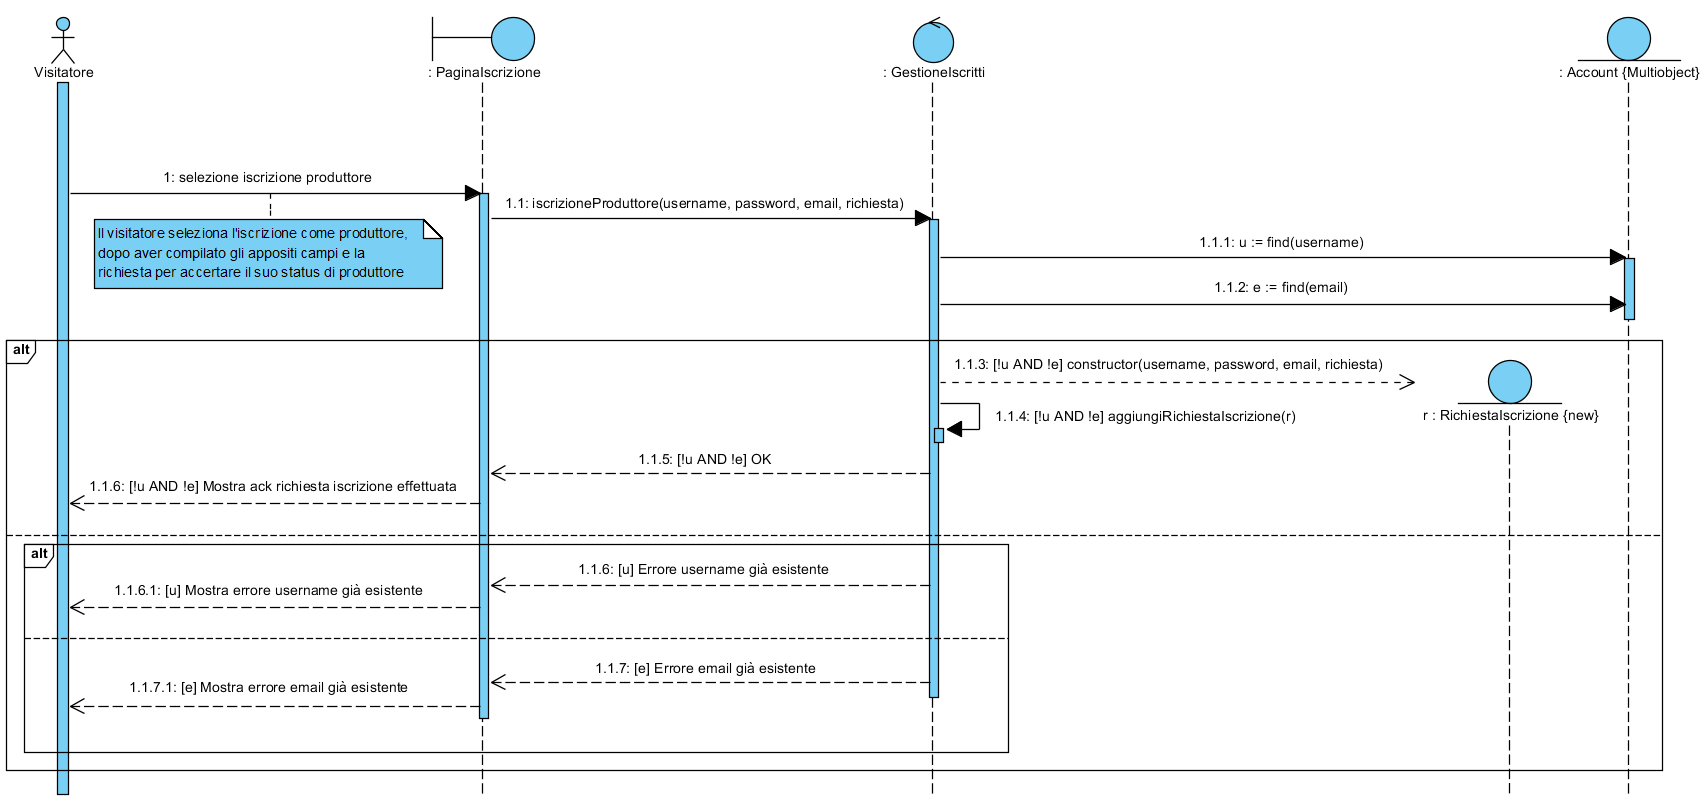
\includegraphics[width=\textwidth]{assets/visualParadigm/sequenza/iscrizioneProduttore}
\end{center}

\linkedSubsection{seq:iscrizioneUtente}
\begin{center}
			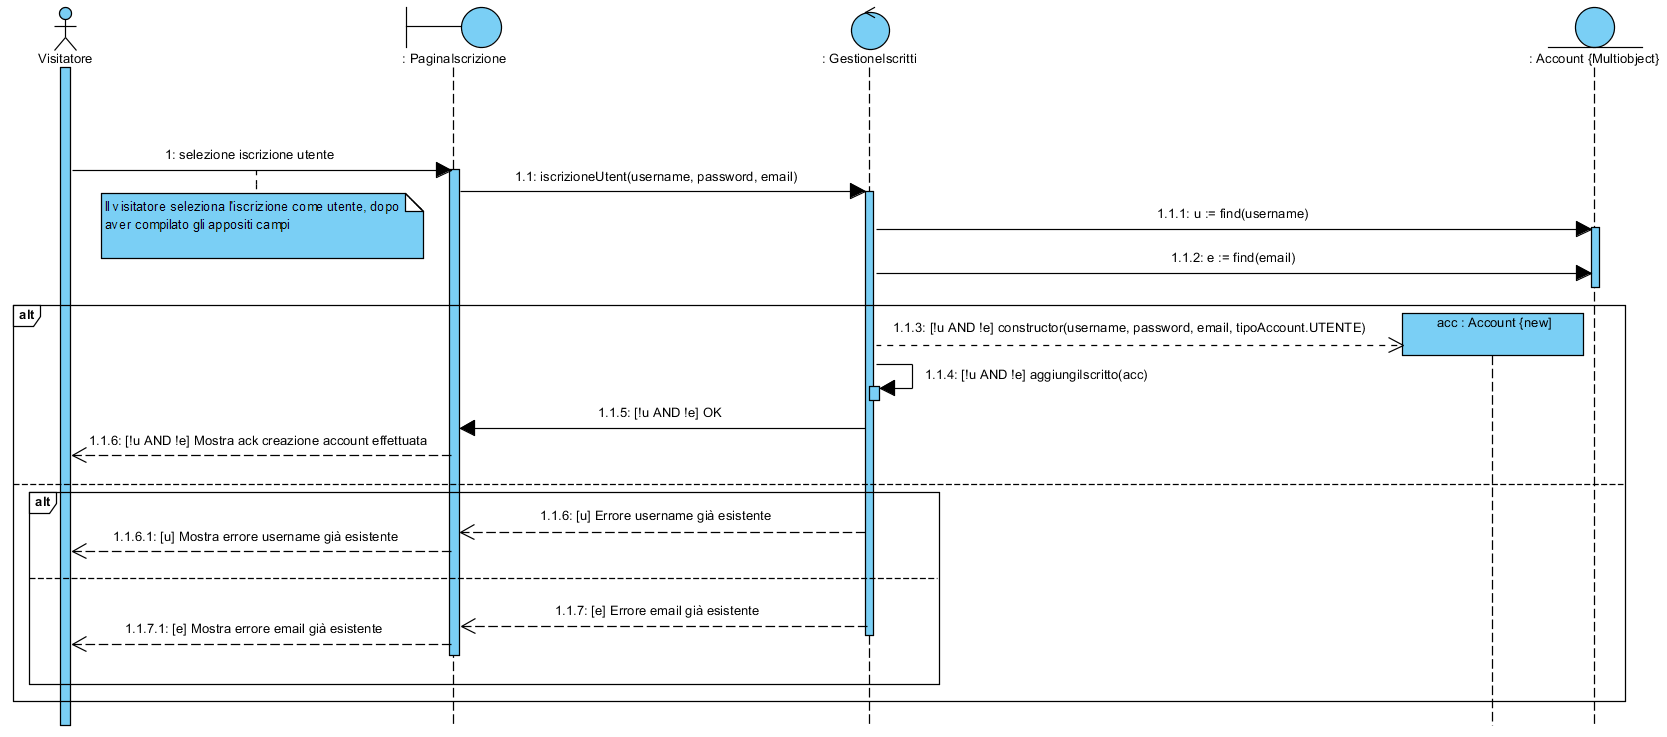
\includegraphics[width=\textwidth]{assets/visualParadigm/sequenza/iscrizioneUtente}
\end{center}

\linkedSubsection{seq:approvazioneIscrizione}
\begin{center}
			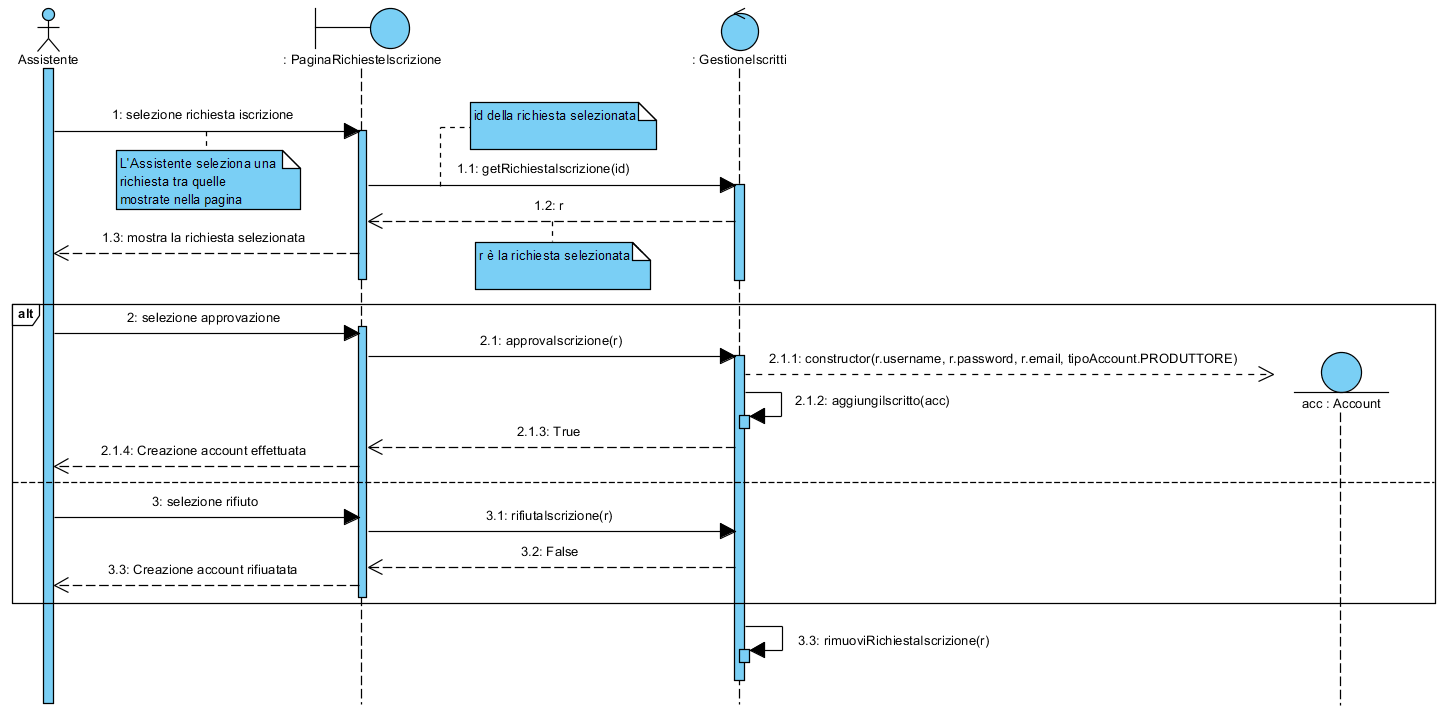
\includegraphics[width=\textwidth]{assets/visualParadigm/sequenza/approvazioneIscrizione}
\end{center}

\linkedSubsection{seq:inserimentoSchedaProdotto}
\begin{center}
			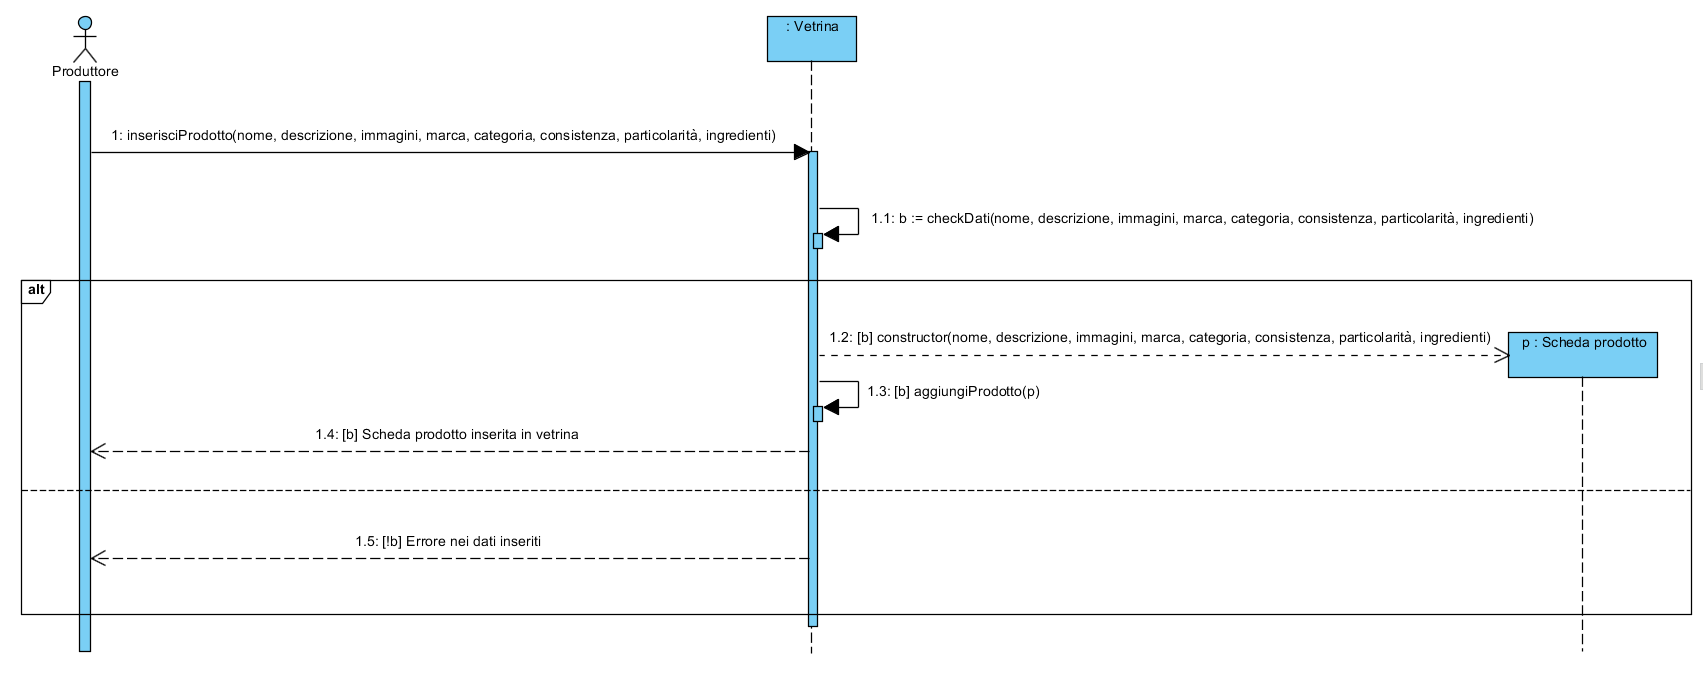
\includegraphics[width=\textwidth]{assets/visualParadigm/sequenza/inserimentoSchedaProdotto}
\end{center}

\linkedSubsection{seq:inserimentoValutazione}
\begin{center}
			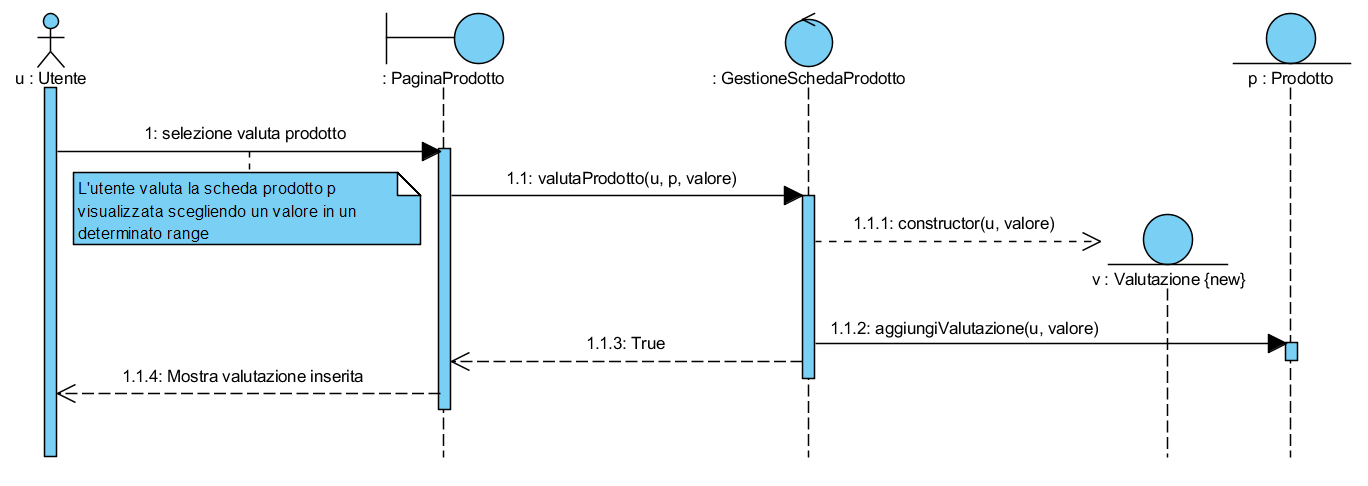
\includegraphics[width=\textwidth]{assets/visualParadigm/sequenza/inserimentoValutazione}
\end{center}

\linkedSubsection{seq:inserimentoRecensione}
\begin{center}
			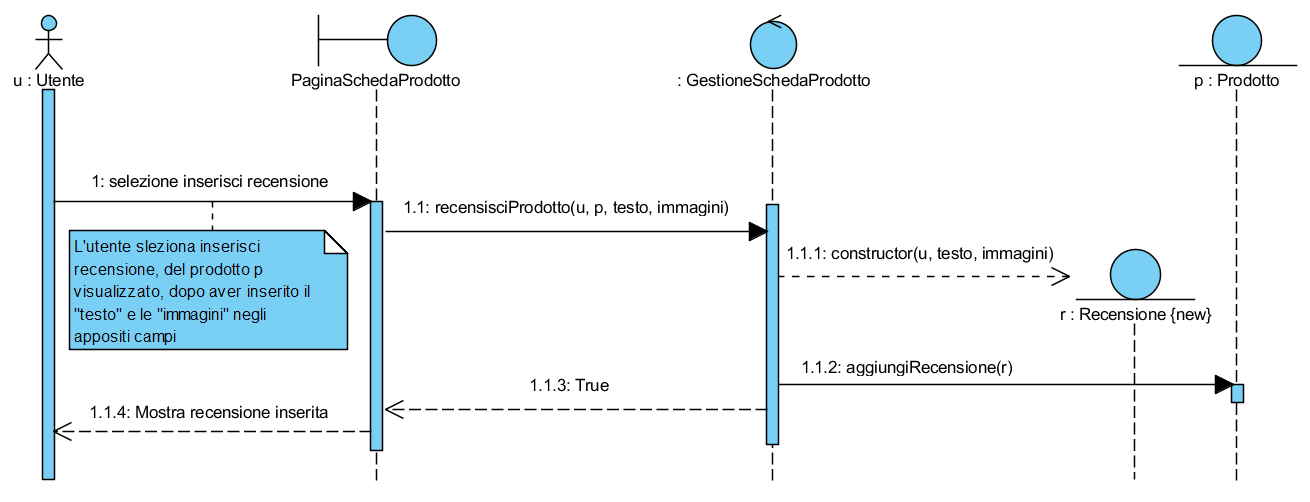
\includegraphics[width=\textwidth]{assets/visualParadigm/sequenza/inserimentoRecensione}
\end{center}

\linkedSubsection{seq:rimuoviRecensione}
\begin{center}
			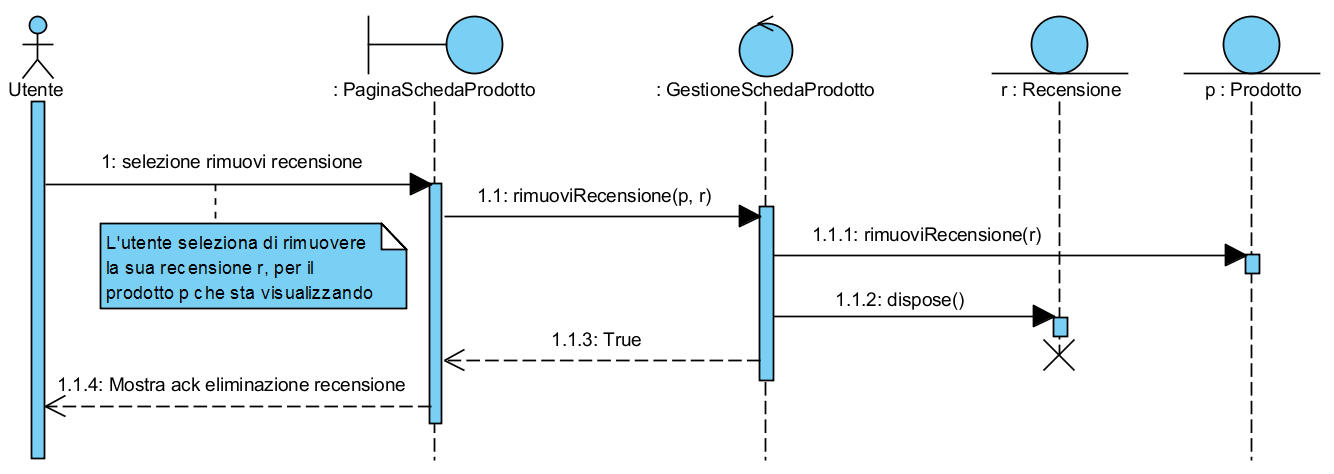
\includegraphics[width=\textwidth]{assets/visualParadigm/sequenza/rimuoviRecensione}
\end{center}

\linkedSubsection{seq:commentoRecensione}
\begin{center}
			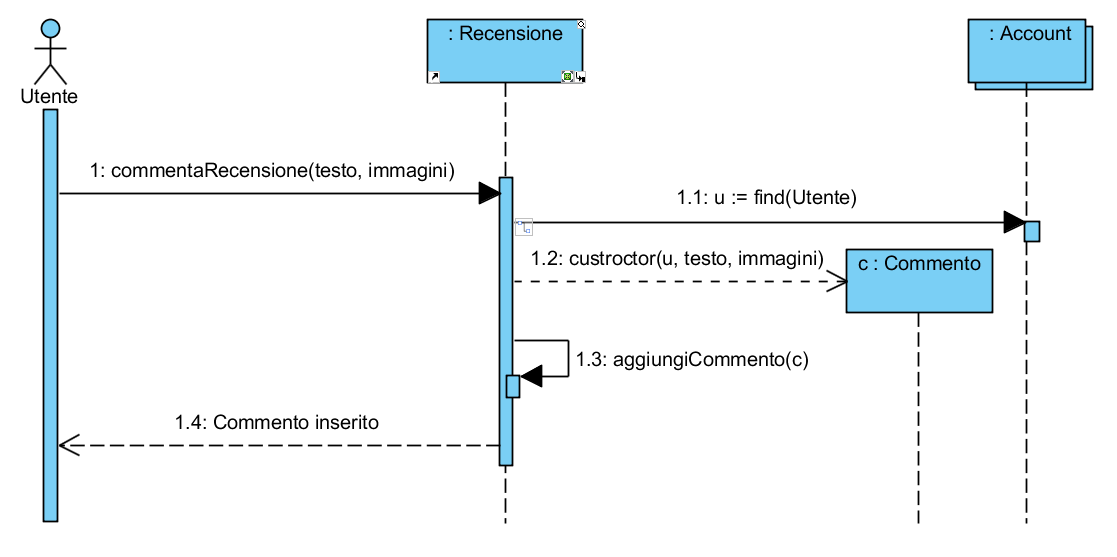
\includegraphics[width=\textwidth]{assets/visualParadigm/sequenza/commentoRecensione}
\end{center}

\linkedSubsection{seq:giudicaRecensione}
\begin{center}
			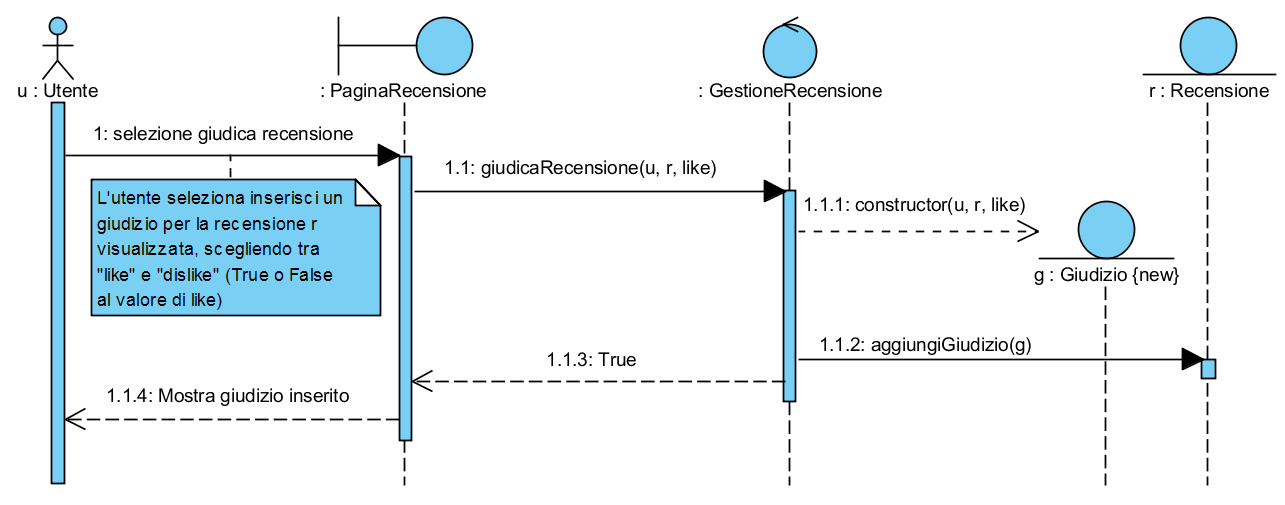
\includegraphics[width=\textwidth]{assets/visualParadigm/sequenza/giudicaRecensione}
\end{center}

\linkedSubsection{seq:ricerca}
\begin{center}
			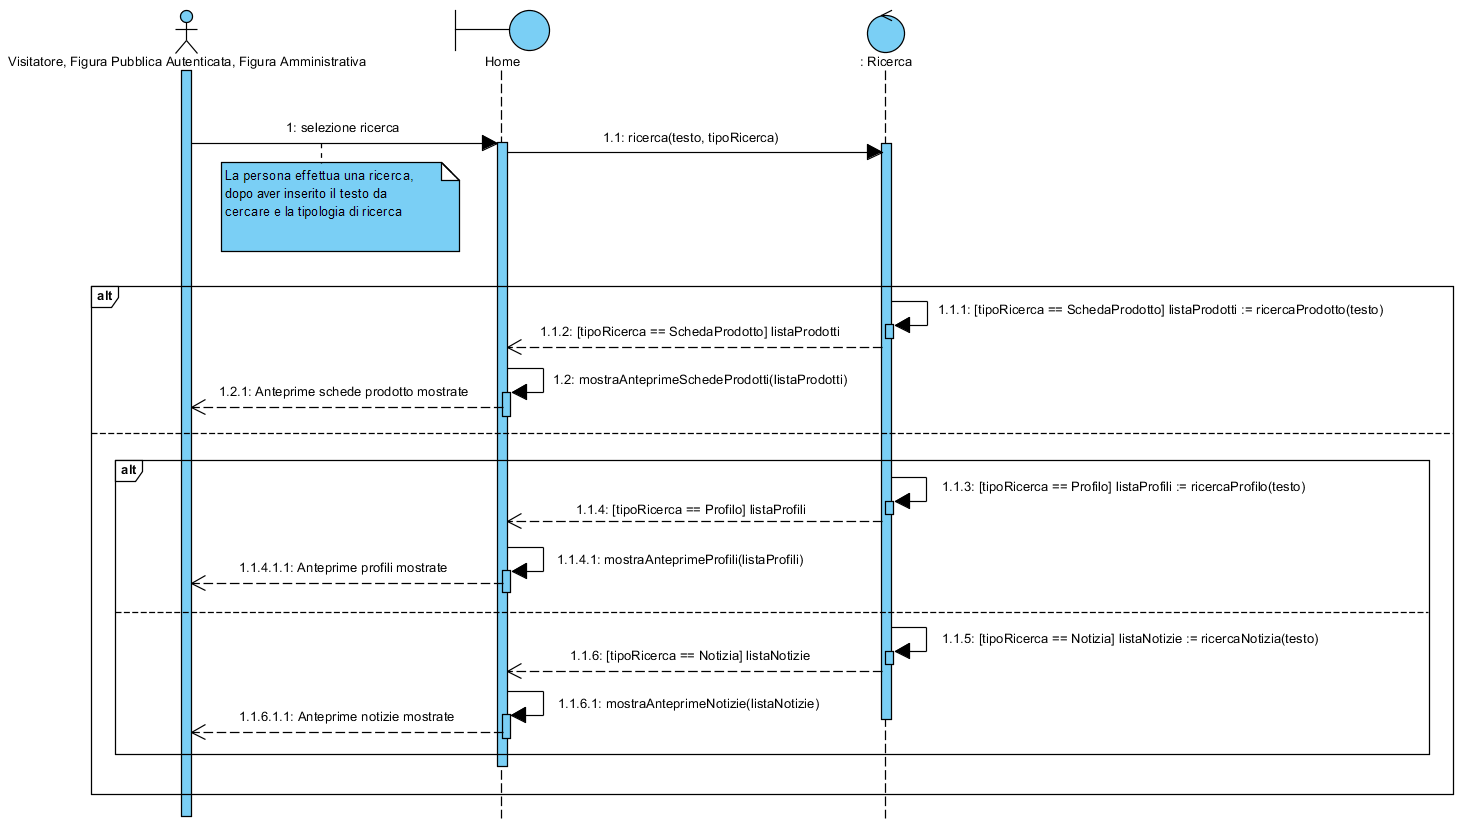
\includegraphics[width=\textwidth]{assets/visualParadigm/sequenza/ricerca}
\end{center}


\newdate{analisiuno}{19}{10}{2016}
\section{Revisioni}
\begin{center}
    \begin{tabular}{lll}
        \toprule
        	\tabhead{Versione} & \tabhead{Data} & \tabhead{Descrizione} \\
		\cmidrule(l{\cmidrulekern}r{\cmidrulekern}){1-3}
        	1.0 & \displaydate{analisiuno} & Prima versione \\
        \bottomrule
    \end{tabular}
\end{center}
